% Digital Logic Report Template
% Created: 2020-01-10, John Miller

%==========================================================
%=========== Document Setup  ==============================

% Formatting defined by class file
\documentclass[11pt]{article}

% ---- Document formatting ----
\usepackage[margin=1in]{geometry}	% Narrower margins
\usepackage{booktabs}				% Nice formatting of tables
\usepackage{graphicx}				% Ability to include graphics

%\setlength\parindent{0pt}	% Do not indent first line of paragraphs 
\usepackage[parfill]{parskip}		% Line space b/w paragraphs
%	parfill option prevents last line of pgrph from being fully justified

% Parskip package adds too much space around titles, fix with this
\RequirePackage{titlesec}
\titlespacing\section{0pt}{8pt plus 4pt minus 2pt}{3pt plus 2pt minus 2pt}
\titlespacing\subsection{0pt}{4pt plus 4pt minus 2pt}{-2pt plus 2pt minus 2pt}
\titlespacing\subsubsection{0pt}{2pt plus 4pt minus 2pt}{-6pt plus 2pt minus 2pt}

% ---- Hyperlinks ----
\usepackage[colorlinks=true,urlcolor=blue]{hyperref}	% For URL's. Automatically links internal references.

% ---- Code listings ----
\usepackage{listings} 					% Nice code layout and inclusion
\usepackage[usenames,dvipsnames]{xcolor}	% Colors (needs to be defined before using colors)

% Define custom colors for listings
\definecolor{listinggray}{gray}{0.98}		% Listings background color
\definecolor{rulegray}{gray}{0.7}			% Listings rule/frame color

% Style for Verilog
\lstdefinestyle{Verilog}{
	language=Verilog,					% Verilog
	backgroundcolor=\color{listinggray},	% light gray background
	rulecolor=\color{blue}, 			% blue frame lines
	frame=tb,							% lines above & below
	linewidth=\columnwidth, 			% set line width
	basicstyle=\small\ttfamily,	% basic font style that is used for the code	
	breaklines=true, 					% allow breaking across columns/pages
	tabsize=3,							% set tab size
	commentstyle=\color{gray},	% comments in italic 
	stringstyle=\upshape,				% strings are printed in normal font
	showspaces=false,					% don't underscore spaces
}

% How to use: \Verilog[listing_options]{file}
\newcommand{\Verilog}[2][]{%
	\lstinputlisting[style=Verilog,#1]{#2}
}




%======================================================
%=========== Body  ====================================
\begin{document}

\title{ELC 2137 Lab 03: Adders}
\author{Kyra Rose}

\maketitle


\section*{Summary}

In this lab we used AND and XOR gate to build circuits that preformed the functions of a half adder, full adder, and a two-bit adder. 


\section*{Q\&A}

1) Which gates could we use for combining the carry bits?

We could use the XOR or the NAND gate. 

2) Which one should we use and why? 

We should use the XOR gate, because we don't want our Cout LED to be one when both carry bits are off. 


\section*{Results}

	\begin{table}[ht]\centering
		\caption{FA Expanded Truth Table}
		\label{tbl:example_table}
		\begin{tabular}{ccc|cccc|cc}
			\toprule
			Cin & A & B & C1 & S1 & C2 & S2 & Cout & S \\
			\midrule
			0 & 0 & 0 & 0 & 0 & 0 & 0 & 0 & 0 \\
			0 & 0 & 1 & 0 & 1 & 0 & 1 & 0 & 1 \\
			0 & 1 & 0 & 0 & 1 & 0 & 1 & 0 & 1 \\
			0 & 1 & 1 & 1 & 0 & 0 & 0 & 1 & 0 \\
			1 & 0 & 0 & 0 & 0 & 0 & 1 & 0 & 1 \\
			1 & 0 & 1 & 0 & 1 & 1 & 0 & 1 & 0 \\
			1 & 1 & 0 & 0 & 1 & 1 & 1 & 1 & 0 \\
			1 & 1 & 1 & 1 & 0 & 0 & 1 & 1 & 1 \\
			\bottomrule
		\end{tabular} 
	\end{table}
\begin{center}
	
	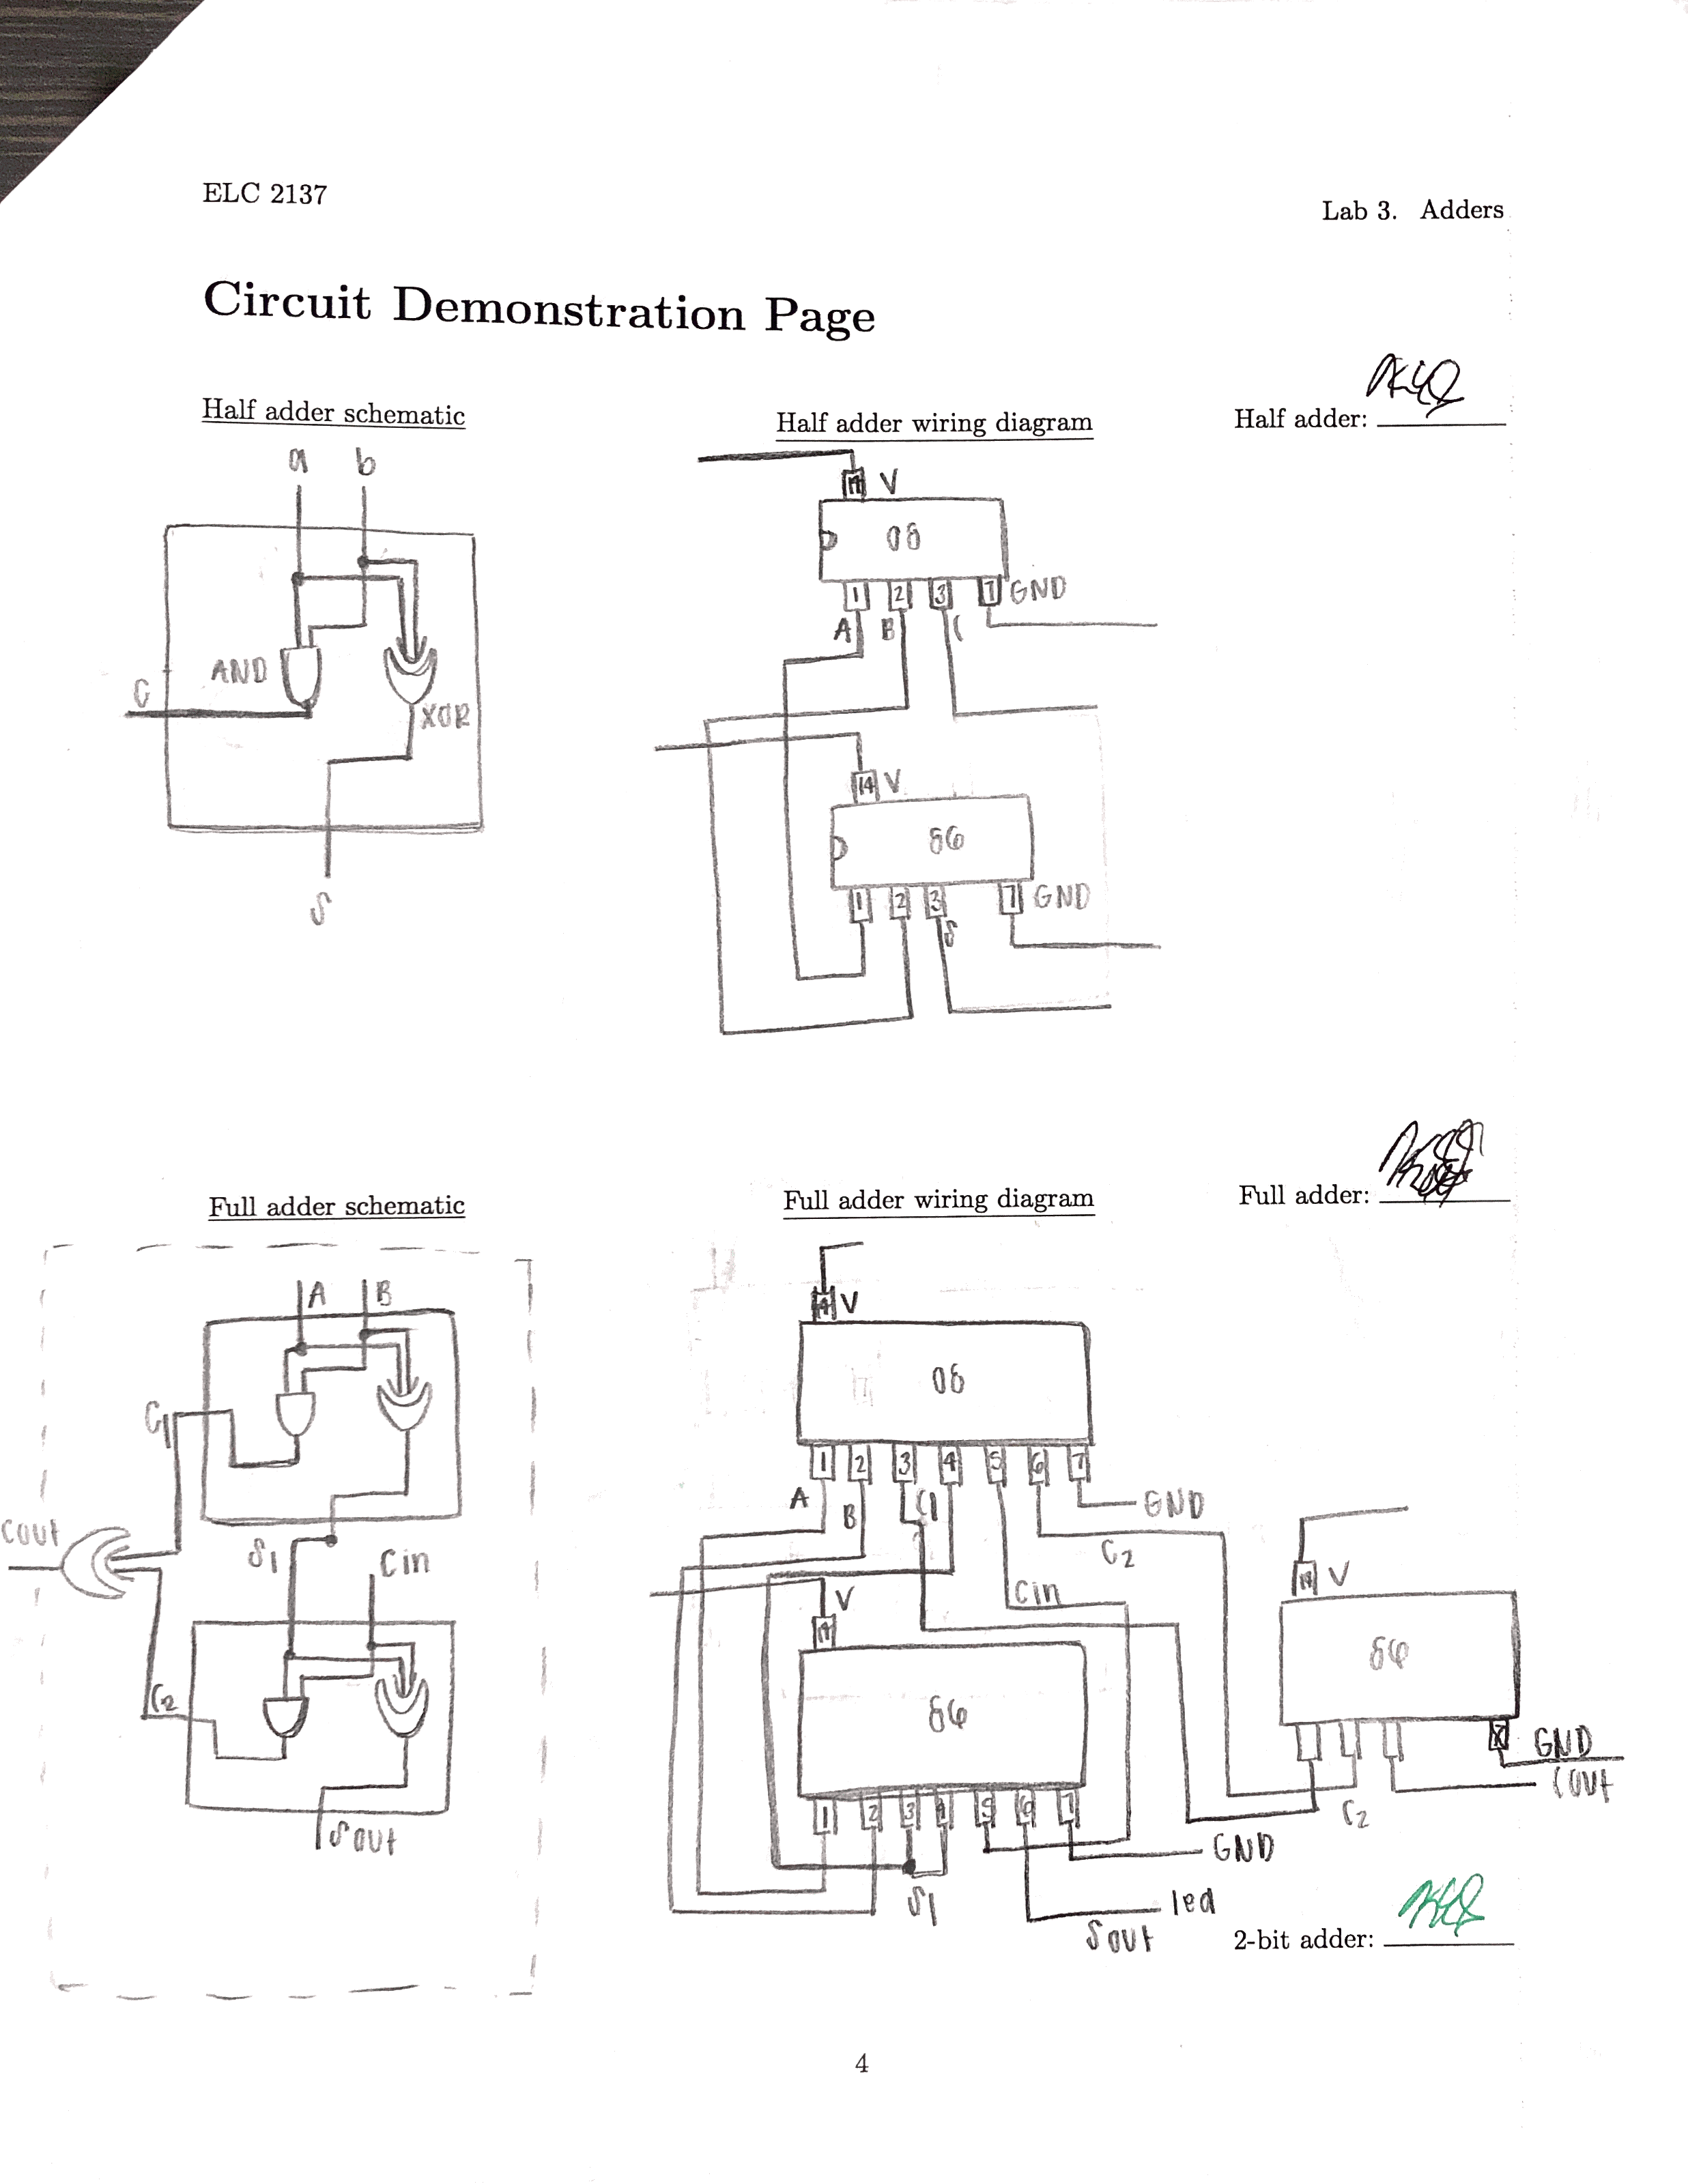
\includegraphics[width=0.5\textwidth]{circuit demo page}
	
	\caption{Circuit Demonstration Page}
	
	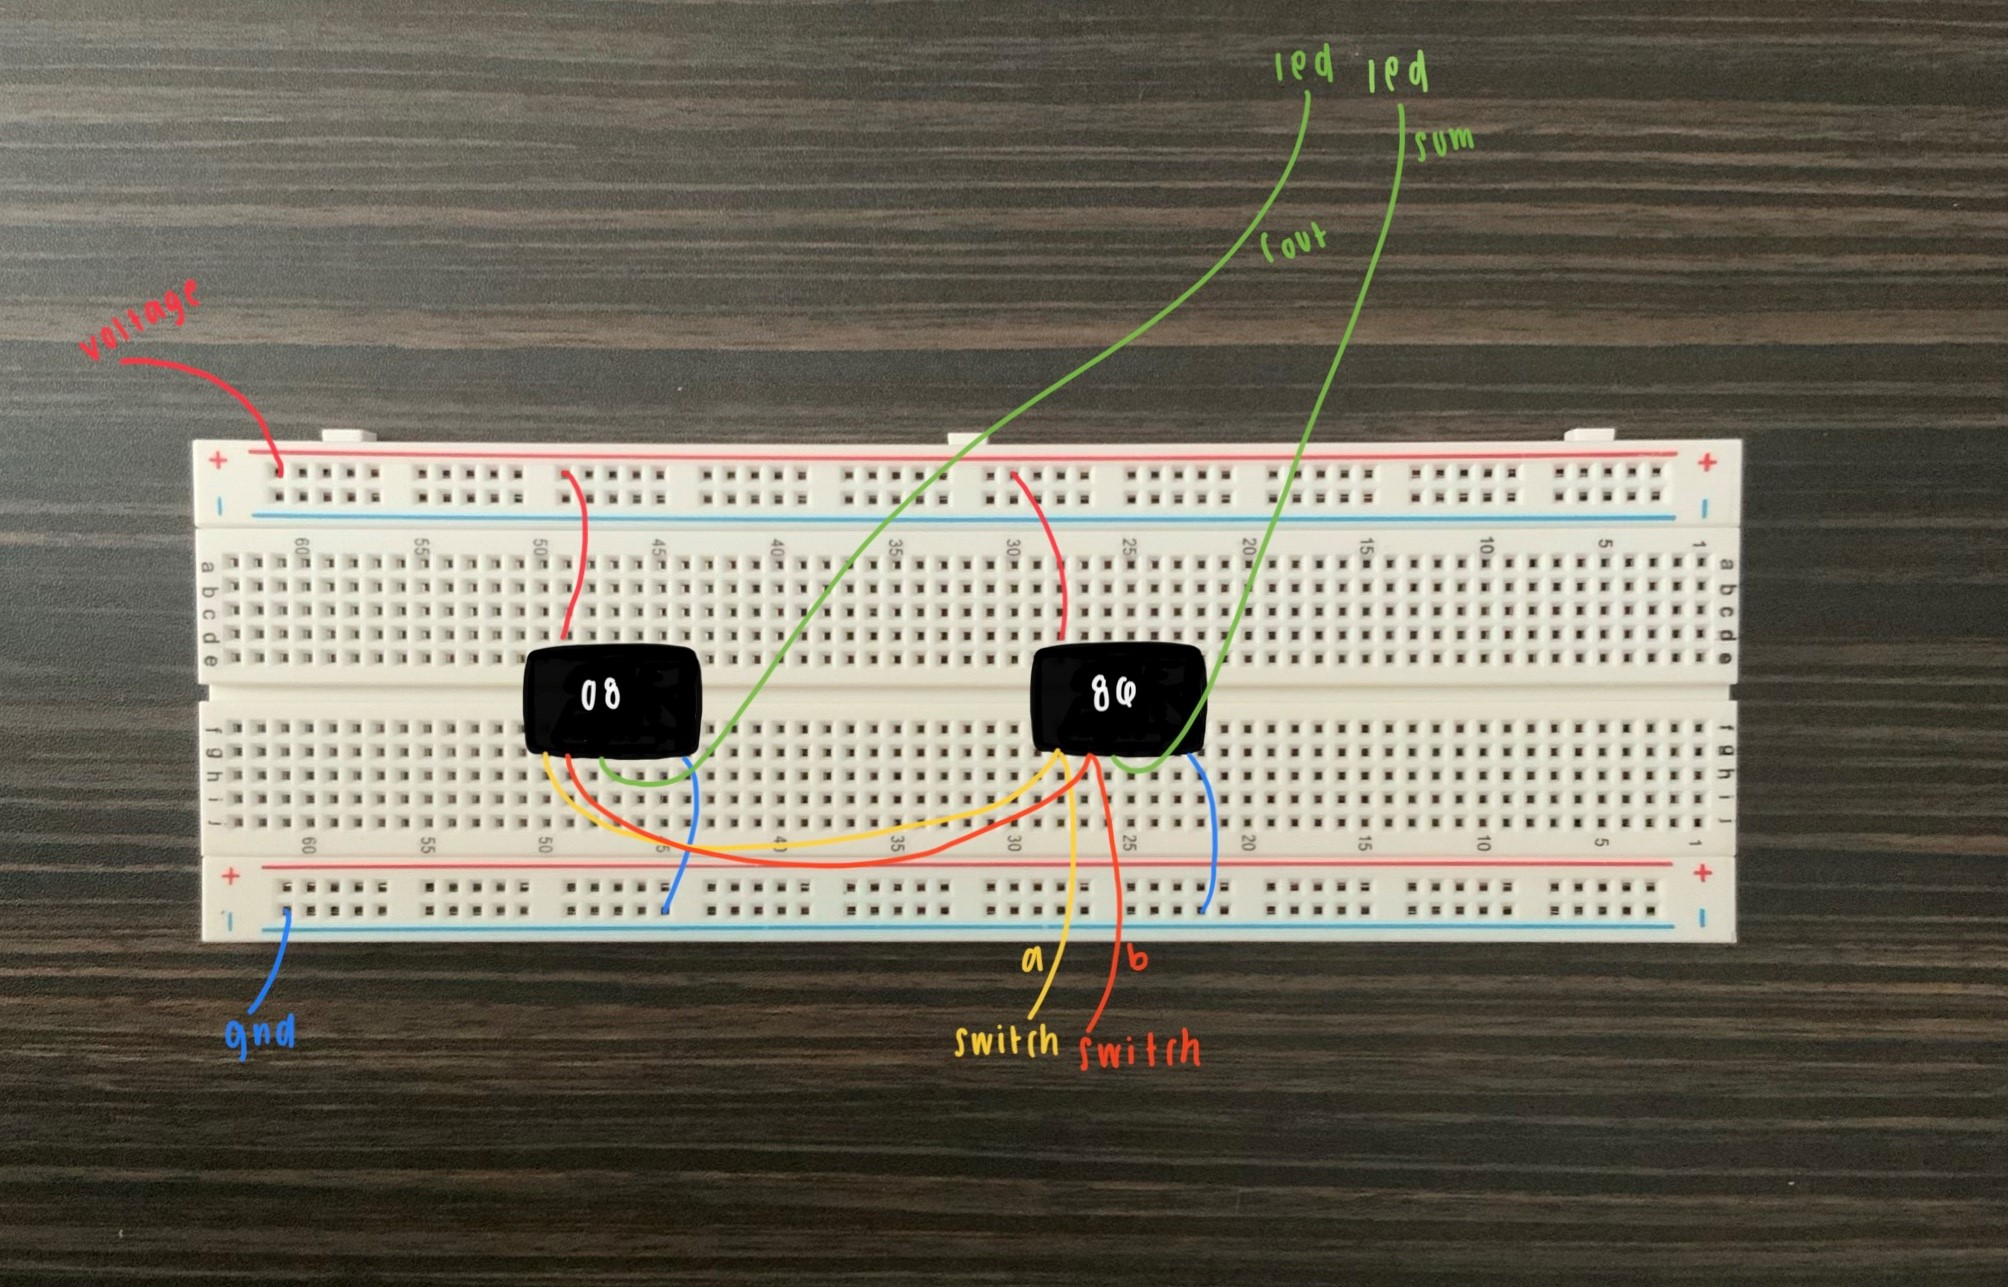
\includegraphics[width=0.5\textwidth]{half adder}
	
	\caption{Half Adder}
	
	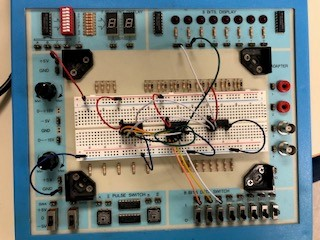
\includegraphics[width=0.5\textwidth]{full adder}
	
	\caption{Full Adder}
	
	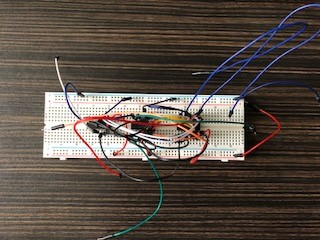
\includegraphics[width=0.5\textwidth]{2 bit adder}
	
	\caption{2 Bit Adder}
	
\end{center}



\section*{Code}

\begin{lstlisting}[style=Verilog,
	caption=Direct Verilog code example,
	label=code:ex 
	]
	\begin{center}
		\caption{Circuit Demonstration Page}
		
		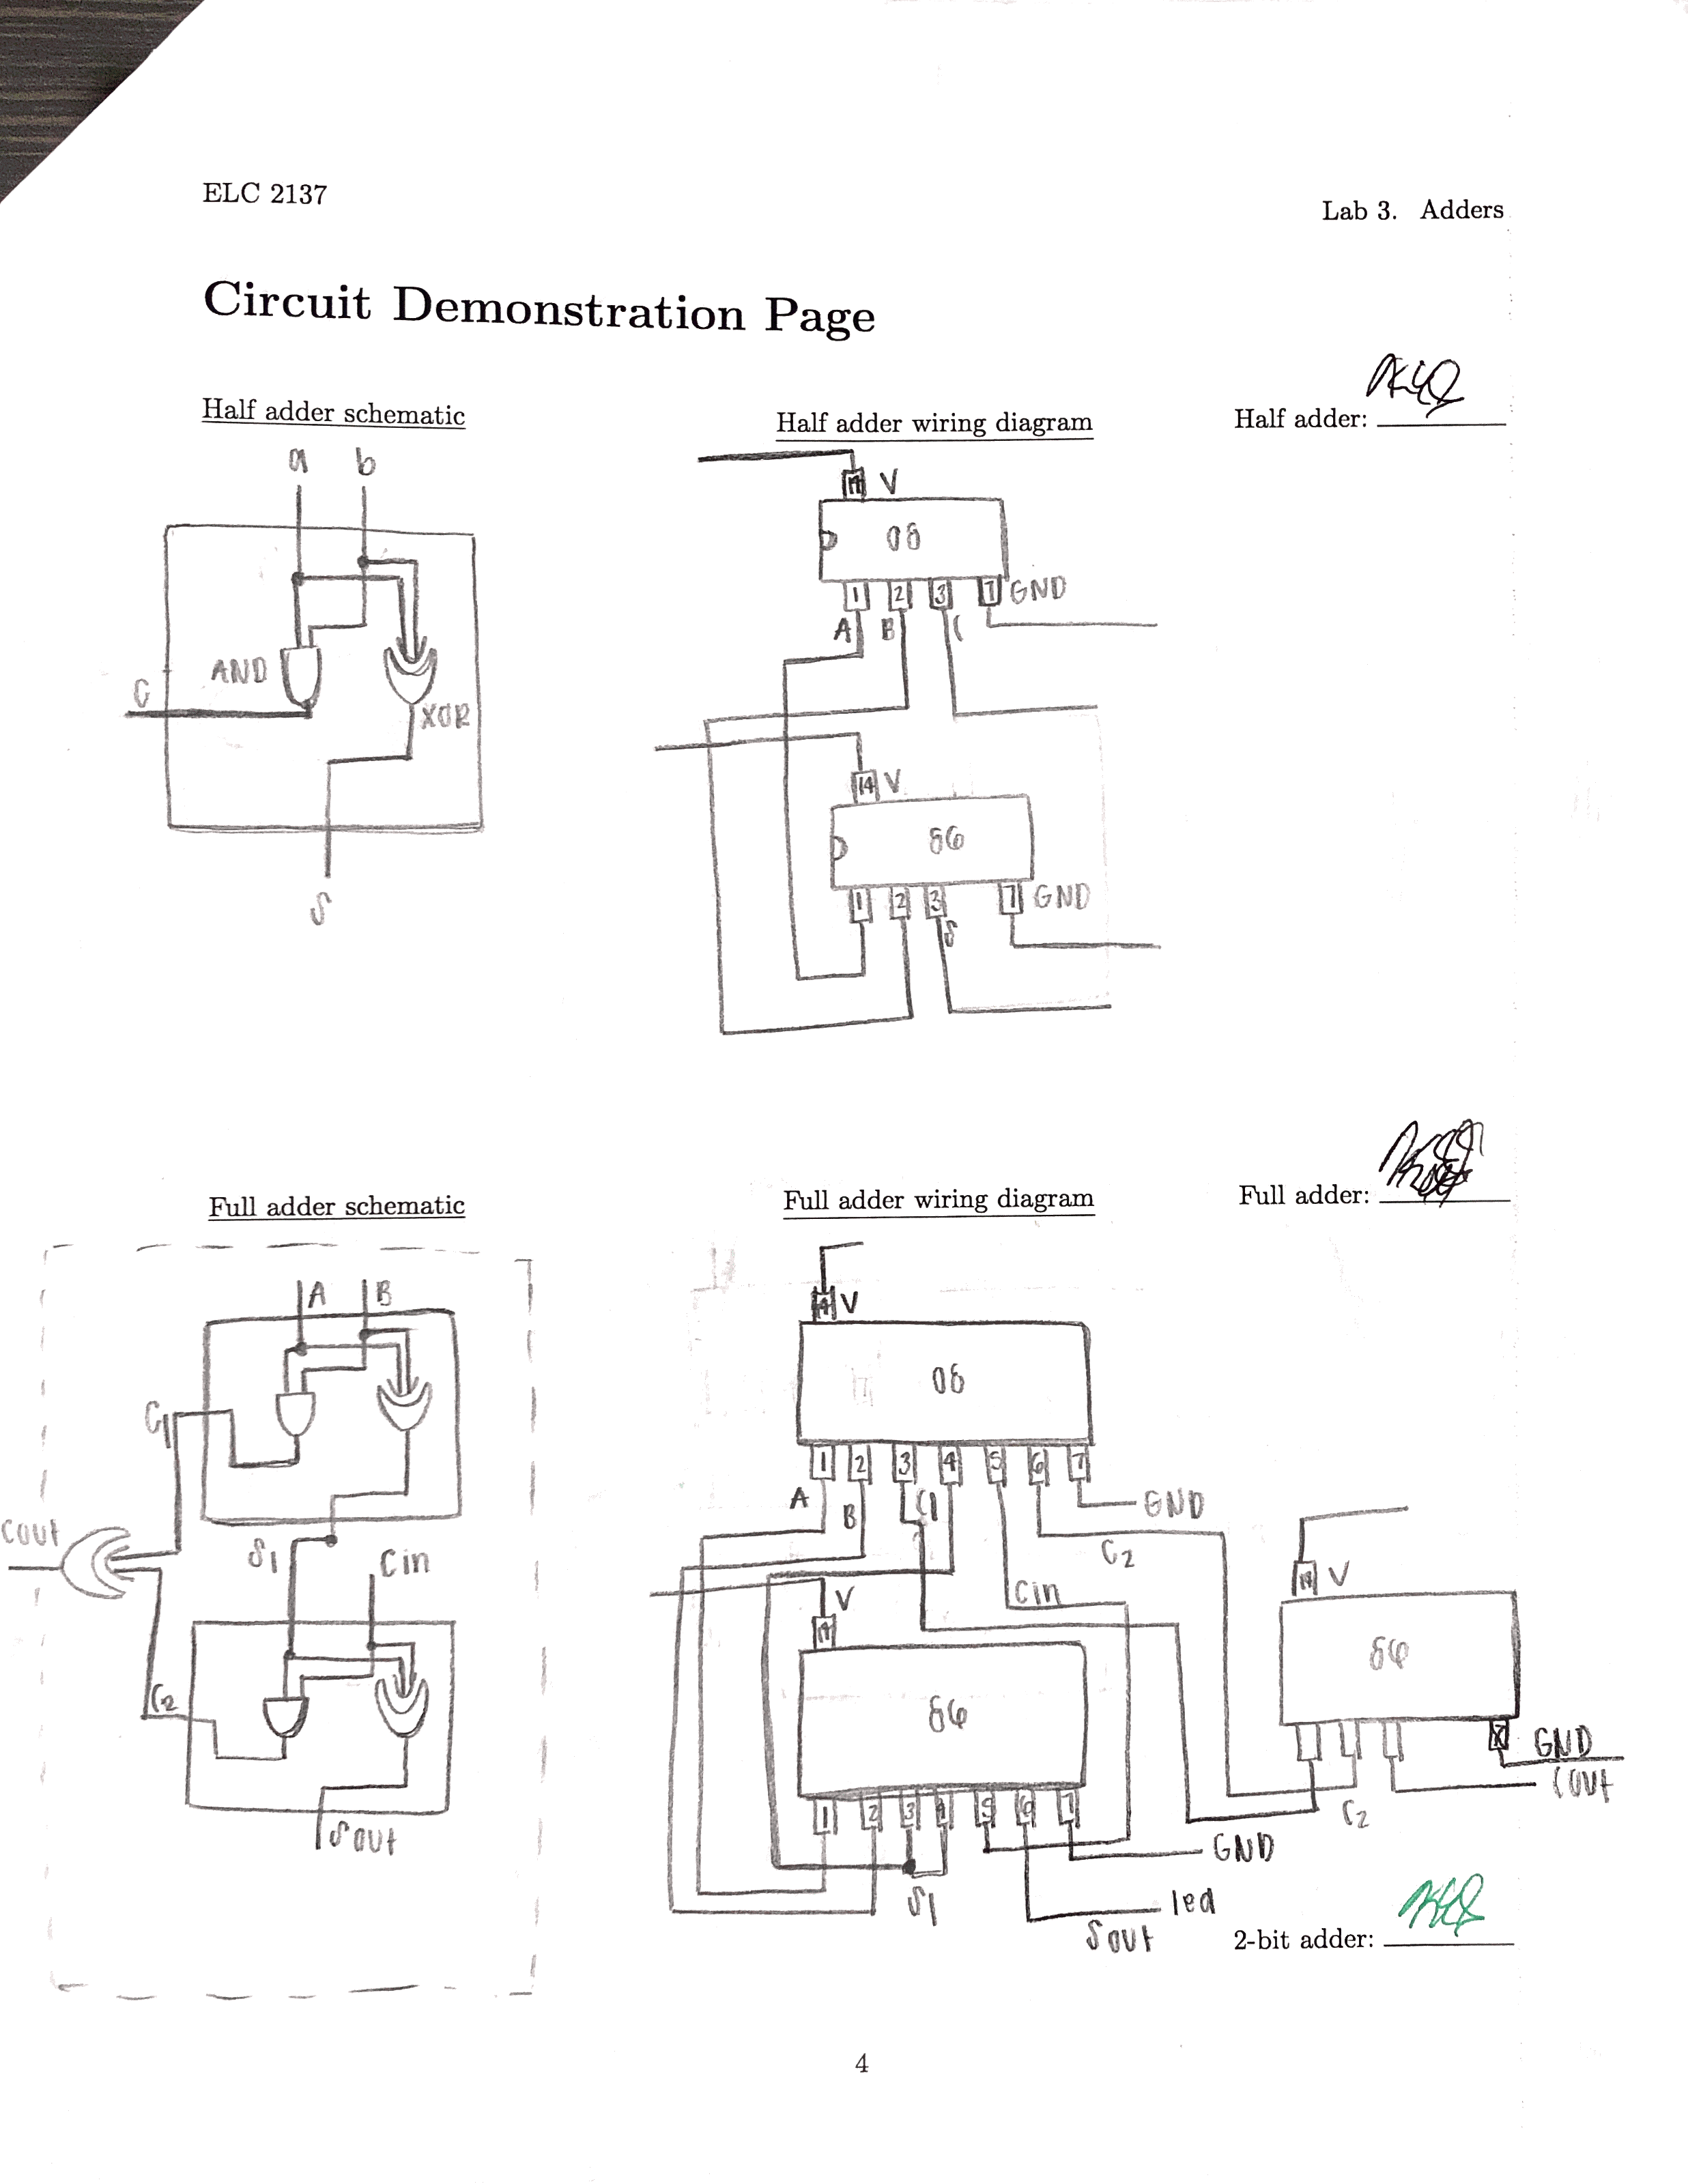
\includegraphics[width=0.5\textwidth]{circuit demo page}
		
		\caption{Half Adder}
		
		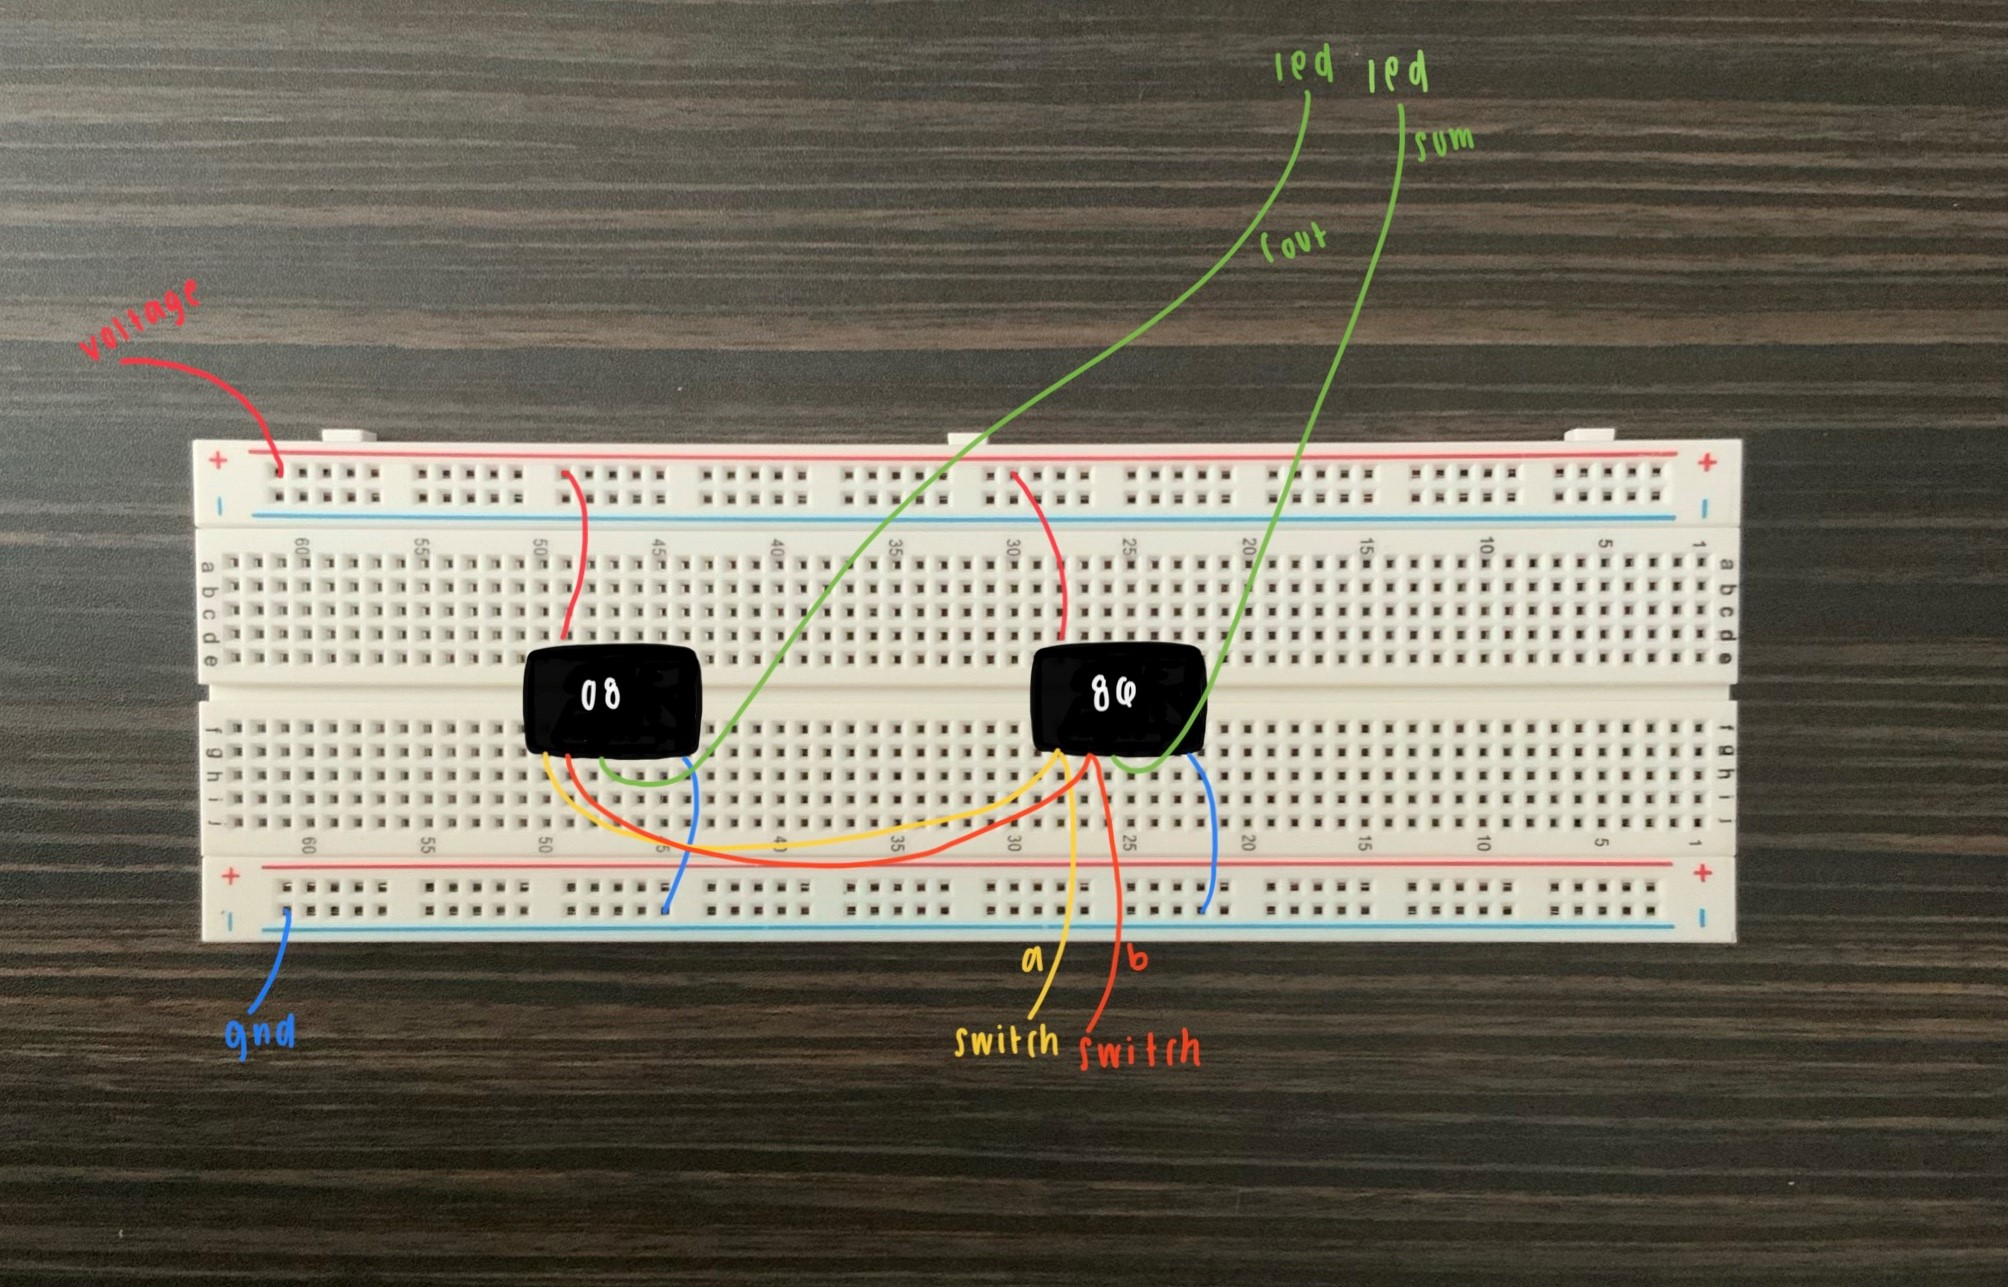
\includegraphics[width=0.5\textwidth]{half adder}
		
		\caption{Full Adder}
		
		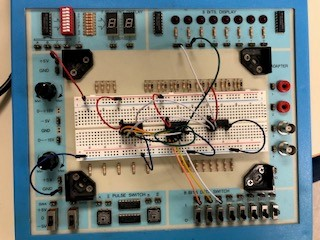
\includegraphics[width=0.5\textwidth]{full adder}
		
		\caption{2 Bit Adder}
		
		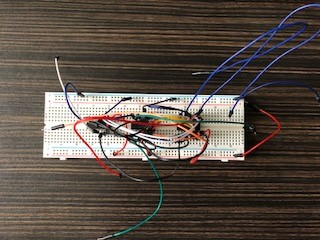
\includegraphics[width=0.5\textwidth]{2 bit adder}
	\end{center}
	
	\begin{table}[ht]\centering
		\caption{FA Expanded Truth Table}
		\label{tbl:example_table}
		\begin{tabular}{ccc|cccc|cc}
			\toprule
			Cin & A & B & C1 & S1 & C2 & S2 & Cout & S \\
			\midrule
			0 & 0 & 0 & 0 & 0 & 0 & 0 & 0 & 0 \\
			0 & 0 & 1 & 0 & 1 & 0 & 1 & 0 & 1 \\
			0 & 1 & 0 & 0 & 1 & 0 & 1 & 0 & 1 \\
			0 & 1 & 1 & 1 & 0 & 0 & 0 & 1 & 0 \\
			1 & 0 & 0 & 0 & 0 & 0 & 1 & 0 & 1 \\
			1 & 0 & 1 & 0 & 1 & 1 & 0 & 1 & 0 \\
			1 & 1 & 0 & 0 & 1 & 1 & 1 & 1 & 0 \\
			1 & 1 & 1 & 1 & 0 & 0 & 1 & 1 & 1 \\
			\bottomrule
		\end{tabular} 
	\end{table}
\end{lstlisting}


\end{document}
